%%%%%%%%%%%%%%%%%%%%%%%%%%%%%%%%%%%%%%%%%%%%%%%%%%%%%%%
%                   File: OSAmeetings.tex             %
%                  Date: 29 Novemver 2018              %
%                                                     %
%     For preparing LaTeX manuscripts for submission  %
%       submission to OSA meetings and conferences    %
%                                                     %
%       (c) 2018 Optical Society of America           %
%%%%%%%%%%%%%%%%%%%%%%%%%%%%%%%%%%%%%%%%%%%%%%%%%%%%%%%

\documentclass[12pt,dvipdfmx]{jsarticle}
%% if A4 paper needed, change letterpaper to A4
\usepackage[dvipdfmx]{graphicx}
\usepackage[dvipdfmx]{color}
\usepackage{osameet3} %% use version 3 for proper copyright statement
\usepackage{ascmac}
%% provide authormark
\newcommand\authormark[1]{\textsuperscript{#1}}

%% standard packages and arguments should be modified as needed
\usepackage{amsmath,amssymb}
\usepackage[colorlinks=true,bookmarks=false,citecolor=blue,urlcolor=blue]{hyperref} %pdflatex
%\usepackage[breaklinks,colorlinks=true,bookmarks=false,citecolor=blue,urlcolor=blue]{hyperref} %latex w/dvipdf
\usepackage{mathtools}
\usepackage{amsmath}
\usepackage{empheq}
\usepackage{physics}
\usepackage[scr=rsfs]{mathalpha}
\usepackage[svgnames]{xcolor}% tikzより前に読み込む必要あり
\usepackage{tikz}
\usepackage{bm}
\usepackage{here}
\usepackage{braket}
\usepackage{framed,color}
\usepackage{dcolumn}
\definecolor{shadecolor}{gray}{0.80}
\usetikzlibrary{perspective}
\tikzset
{%
  my ball/.style={draw,circle,minimum size=2*\r cm,inner sep=0,shading=ball,ball color=cyan!50!blue,opacity=#1},
  my ball/.default=1,
  hidden line/.style={black!60}
}
\begin{document}
\title{東大物理工学科 2014}

\author{21B00817 鈴木泰雅,\authormark{1}}
\section*{\Large{第一問}}
\subsection*{\large{[1]}}
\begin{eqnarray}
  \int r^2 \rho dm &&= \frac{m}{\frac{4}{3}\pi a^3}\int_{-a}^{a} \int_0^\pi\int_0^{\sqrt{r^2-z^2}}((a^2-x^2)xdx) d\theta dz\\
  &&= \frac{2}{5}ma^2
\end{eqnarray}
となる.
\subsection*{\large{[2]}}
滑らないという条件から,
\begin{eqnarray}
  v' = -a\omega'
\end{eqnarray}
となる.
\subsection*{\large{[3]}}
線形運動量と角運動量の保存より
\begin{eqnarray}
  mv'-o =P,\quad aP = \frac{2}{5}ma^2(\omega'-\omega)
\end{eqnarray}
であり,これを解いて
\begin{eqnarray}
  \omega' = \frac{2}{7}\omega
\end{eqnarray}
\subsection*{\large{[4]}}
線形運動量と角運動量の保存より
\begin{eqnarray}
  P_n = mv_n - mv_{n-1}, \quad P_n a = \frac{2}{5}ma^2 (\omega_n-\omega_{n-1})
\end{eqnarray}
である.よって,
\begin{eqnarray}
  I(\omega_n-\omega_{n-1})- a(mv_n - mv_{n-1})=0, \quad\therefore (I\omega_n-amv_n) = (I\omega_{n-1}-amv_{n-1})
\end{eqnarray}
よって,
\begin{eqnarray}
  (I\omega_n-amv_n) = (I\omega_{n-1}-amv_{n-1}) = \cdots (I\omega_{0}-amv_{0}) = \text{Const}
\end{eqnarray}
より,
\begin{eqnarray}
  l = I\omega_n-amv_n  = \text{Const}
\end{eqnarray}
\subsection*{\large{[5]}}
反発が終わった直後では,
\begin{eqnarray}
  \omega_f = \frac{v_f}{a}
\end{eqnarray}
の関係が成立するため,
\begin{eqnarray}
  l = I \frac{v_f}{a} - ma v_f , \quad\therefore v_f = \frac{5l}{3ma}
\end{eqnarray}
である.\\
また,$v_f=0$のとき,$l=0$であるため,
\begin{eqnarray}
  I\omega_0 -mav_0=0,\quad\therefore \frac{2}{5}ma\omega_0 = mv_0
\end{eqnarray}
\newpage
\section*{\Large{第二問}}
\subsection*{\large{[1]}}
電場の大きさはガウスの法則より
\begin{eqnarray}
  E(r)\cdot 2\pi r l = \frac{1}{\epsilon_0}\lambda l,\quad\therefore E(r) = \frac{\lambda}{2\pi r \epsilon_0}
\end{eqnarray}
である.また,電位は
\begin{eqnarray}
  \phi(r)-\phi(r_0) = \phi(r) = -\int_{r_0}^{r} E(r) dr = -\frac{\lambda}{2\pi\epsilon_0}\log\frac{r}{r_0}
\end{eqnarray}
\subsection*{\large{[2]}}
上記の表式から見て分かるように,ポテンシャルは,線素からの距離$r$のみしか依存しない.また,重ね合わせの原理から
\begin{eqnarray}
  \phi&&= \phi_{\lambda} + \phi_{-\lambda} = \frac{\lambda}{2\pi\epsilon_0}\left( -\log \frac{\sqrt{a^2+r^2-2ar\cos\theta}}{r_0}+\log \frac{\sqrt{b^2+r^2-2br\cos\theta}}{r_0} \right)\\
  &&= \frac{\lambda}{4\pi\epsilon_0}\log\left( \frac{b^2 + r^2 -2br\cos\theta}{a^2 + r^2 -2ar\cos\theta} \right)
\end{eqnarray}
\subsection*{\large{[3]}}
必要条件であるため,代入して一定になることを確かめるだけでは十分ではない.逆を示す必要がある.$\phi$が$r=R$で$\theta$の依存性がない時,
\begin{eqnarray*}
  D^2 + R^2 -2DR\cos\theta = C(d^2 + R^2 -2dR\cos\theta), \quad\therefore d^2\left[ C^2+C(-1-(R/d)^2) + (R/d)^2 \right] + 2R\cos\theta(Cd-D)=0
\end{eqnarray*}
であり.これが恒等的に成立するための条件は
\begin{eqnarray}
  C = \frac{D}{d}, C= (R/d)^2,1 \quad\therefore D = \frac{R^2}{d}, d
\end{eqnarray}
であり,$D\neq d$であるため,
\begin{eqnarray}
  D = \frac{R^2}{d}
\end{eqnarray}
となる.
\subsection*{\large{[4]}}
これをもとに計算すると
\begin{eqnarray}
  \sigma(\theta) = \frac{\lambda}{4\pi}\left( -\frac{2}{R} \right)\frac{1-(d/R)^2}{1-2(d/R)\cos\theta + (d/R)^2}
\end{eqnarray}
である.
\subsection*{\large{[5]}}
球面上で積分すると
\begin{eqnarray}
  \int \sigma(\theta)dS &&= \int_{-\pi}^{\pi} \sigma(\theta) Rd\theta =  \frac{\lambda}{4\pi}\left( -\frac{2}{R} \right) R\int_{-\pi}^{\pi} \left[ 1+2\sum_{n=1}^{\infty}{(d/R)}^{n}\cos(n\theta) \right]d\theta\\
  &&= \frac{\lambda}{4\pi} (-2/R) R 2\pi = -\lambda
\end{eqnarray}
よって示せた.
\subsection*{\large{[6]}}
$\sigma_2$の位置は$\theta=\pi/2-\psi$であり,まとめると
\begin{eqnarray}
  &&\sigma_1 : \theta=-\psi\\
  &&\sigma_2 : \theta=\pi/2-\psi\\
  &&\sigma_3 : \theta=\pi-\psi\\
  &&\sigma_4 : \theta=3\pi/2-\psi
\end{eqnarray}
であり,$cos(\theta+\pi)=-\cos\theta$であり,
\begin{eqnarray}
  \frac{\sigma_1}{\sigma_3} = \frac{1+2(d/R)\cos\psi + (d/R)^2}{1-2(d/R)\cos\psi + (d/R)^2} \sim \frac{1+2(d/R)\cos\psi}{1-2(d/R)\cos\psi},\quad\therefore d\cos\psi= \frac{\sigma_1-\sigma_3}{\sigma_1+\sigma_3}\frac{1}{2}R
\end{eqnarray}
となる.また,同様にして
\begin{eqnarray}
  \frac{\sigma_2}{\sigma_4} = \frac{1+2(d/R)\sin\psi + (d/R)^2}{1-2(d/R)\sin\psi + (d/R)^2}\quad\therefore d\sin\psi= \frac{\sigma_2-\sigma_4}{\sigma_2+\sigma_4}\frac{1}{2}R 
\end{eqnarray}
よって,
\begin{eqnarray}
  (x_0,y_0) = \left( \frac{\sigma_1-\sigma_3}{\sigma_1+\sigma_3}\frac{1}{2}R, \frac{\sigma_2-\sigma_4}{\sigma_2+\sigma_4}\frac{1}{2}R  \right)
\end{eqnarray}
\newpage
\section*{\Large{第三問}}
\subsection*{\large{[1]}}
\begin{eqnarray}
  \psi_S: -J ,\quad \psi_A: J
\end{eqnarray}
である.(後の問題と辻褄を合わせるため,理由は分からない.)
\subsection*{\large{[2]}}
波動関数は実関数であるため,
\begin{eqnarray}
  \int_{-\infty}^{\infty} \psi^{*}_L(x)\psi_R(x)dx &&= \frac{1}{2}\int_{-\infty}^{\infty} \left( \psi^{*}_S + \psi^{*}_A \right)\left( \psi_S - \psi_A \right)dx\\
  &&= \frac{1}{2}\int_{-\infty}^{\infty} \left( \psi_S^2 - \psi^2_A + \psi_A\psi_S - \psi_S \psi_A \right)dx = \frac{1}{2}\int_{-\infty}^{\infty} \left( \psi_S^2 - \psi^2_A\right)dx 
\end{eqnarray}
ここでグラフより
\begin{eqnarray}
  \psi_S^2 - \psi^2_A =0
\end{eqnarray}
より,
\begin{eqnarray}
  \int_{-\infty}^{\infty} \psi^{*}_L(x)\psi_R(x)dx=0
\end{eqnarray}
であるため直交している.\\
また,
\begin{eqnarray}
  H \psi_L(x) = -J\psi_R(x),\quad H \psi_R(x) = -J\psi_L(x)
\end{eqnarray}
であり,
\begin{eqnarray}
  |\psi_L\rangle=
  \begin{bmatrix}
    1\\
    0
  \end{bmatrix},\quad
  |\psi_R\rangle=
  \begin{bmatrix}
    0\\
    1
  \end{bmatrix}
\end{eqnarray}
とすると,
\begin{eqnarray}
  H = -J
  \begin{bmatrix}
    0 & 1\\
    1 & 0
  \end{bmatrix}
  =-J\sigma_x
\end{eqnarray}
\subsection*{\large{[3]}}
\begin{eqnarray}
  |\psi(t)\rangle &&= \exp\left( -i\frac{-J\sigma_x}{\hbar}t \right)|\psi_L\rangle =
  \left( \cos(-Jt/\hbar)\sigma_I-i\sin(-Jt/\hbar)\sigma_X \right)
  \begin{bmatrix}
    1\\
    0
  \end{bmatrix}\\
  &&=
  \begin{bmatrix}
    \cos(-Jt/\hbar) & -i\sin(-Jt/\hbar)\\
    -i\sin(-Jt/\hbar) & \cos(-Jt/\hbar)
  \end{bmatrix}
  \begin{bmatrix}
    1\\
    0
  \end{bmatrix}\\
  &&= 
  \begin{bmatrix}
    \cos(-Jt/\hbar)\\
    -i\sin(-Jt/\hbar)
  \end{bmatrix}
\end{eqnarray}
となり,確率は
\begin{eqnarray}
  |\langle \psi_R| \psi(t)\rangle|^2 = \sin^2(-Jt/\hbar)
\end{eqnarray}
\subsection*{\large{[4.1]}}
それぞれの粒子を合成して,まず,二つの粒子が左にいる場合は
\begin{eqnarray}
  |0\rangle = |\psi_L\rangle|\psi_L\rangle
\end{eqnarray}
と表記する.ここで,ハミルトニアンは粒子1と粒子2それぞれに対する作用の和で書けるため,
\begin{eqnarray}
  H = H_1 + H_2
\end{eqnarray}
となる.よって,
\begin{eqnarray}
  H |\psi_L\rangle|\psi_L\rangle = (H_1|\psi_L\rangle)|\psi_L\rangle + |\psi_L\rangle(H_2|\psi_L\rangle) = -J( |\psi_R\rangle|\psi_L\rangle+ |\psi_L\rangle|\psi_R\rangle )
\end{eqnarray}
である.ここで,ボーズ粒子を考えているため
\begin{eqnarray}
  |1\rangle = \frac{1}{\sqrt{2}}( |\psi_R\rangle|\psi_L\rangle+ |\psi_L\rangle|\psi_R\rangle )
\end{eqnarray}
より,
\begin{eqnarray}
  H|0\rangle = -\sqrt{2}J|1\rangle
\end{eqnarray}
であり,
\begin{eqnarray}
  H|1\rangle &&=\frac{1}{\sqrt{2}} \left[ (H_1|\psi_R\rangle)|\psi_L\rangle +|\psi_R\rangle(H_2|\psi_L\rangle)+(H_1|\psi_L\rangle)|\psi_R\rangle +|\psi_L\rangle(H_2|\psi_R\rangle) \right]\\
  &&=  -J\frac{1}{\sqrt{2}} \left[ 2|\psi_L\rangle|\psi_L\rangle + 2|\psi_R\rangle|\psi_R\rangle \right] = -\sqrt{2}J|1\rangle -\sqrt{2}J|2\rangle
\end{eqnarray}
となり,同様にして
\begin{eqnarray}
  H|2\rangle =  -\sqrt{2}J|1\rangle
\end{eqnarray}
となる.よって,
\begin{eqnarray}
  |0\rangle =
  \begin{bmatrix}
    1\\
    0\\
    0
  \end{bmatrix},\quad
  |1\rangle =
  \begin{bmatrix}
    0\\
    1\\
    0
  \end{bmatrix},\quad
  |2\rangle =
  \begin{bmatrix}
    0\\
    0\\
    1
  \end{bmatrix}
\end{eqnarray}
とするとたしかに与えられた行列を得る.
\subsection*{\large{[4.2]}}
この固有値を求めれば良い.よって,
\begin{eqnarray}
  \det
  \begin{bmatrix}
    \lambda & \sqrt{2}J & 0\\
    \sqrt{2}J & \lambda & \sqrt{2}J\\
    0 & \sqrt{2}J & \lambda
  \end{bmatrix}
  =0
\end{eqnarray}
より,$0,\pm 2J$
となる.
\subsection*{\large{[4.3]}}
\begin{eqnarray}
  |\psi(t)\rangle &&= \exp( -iHt/\hbar )|0\rangle = \left( \sum_{n=0}^{\infty}\frac{1}{n!}(-iHt/\hbar)^n  \right)|0\rangle\\
  &&= \left( \sum_{n=0}^{\infty}\frac{1}{(2n)!}(-iHt/\hbar)^{2n} + \sum_{n=0}^{\infty}\frac{1}{(2n+1)!}(-iHt/\hbar)^{2n+1} \right)|0\rangle
\end{eqnarray}
であり,
\begin{eqnarray}
  A:= 
  \begin{bmatrix}
    0 & 1& 0\\
    1 & 0 & 1\\
    0 & 1& 0
  \end{bmatrix},\quad
  B:=
  \begin{bmatrix}
    1 & 0 & 1\\
    0 & 2& 0\\
    1 & 0 & 1
  \end{bmatrix}
\end{eqnarray}
とする.ここで,
\begin{eqnarray}
  A^{2n+1} = 2^nA, \quad A^{2n} = A A^{2n-1} = 2^{n-1}A^2 = 2^{n-1}B 
\end{eqnarray}
であることを利用して
\begin{eqnarray}
  \sum_{n=0}^{\infty}\frac{1}{(2n)!}(-iHt/\hbar)^{2n} &&= I + \sum_{n=1}^{\infty} \frac{1}{(2n)!}(-1)^n (-\sqrt{2}J t/\hbar)^{2n}2^{n-1} B\\
  &&= I + \frac{1}{2}\sum_{n=1}^{\infty} \frac{1}{(2n)!}(-1)^n (-2J t/\hbar)^{2n} B\\
  &&= I + \frac{1}{2}\left( \cos(-2J t/\hbar)-1 \right)B\\
  \sum_{n=0}^{\infty}\frac{1}{(2n+1)!}(-iHt/\hbar)^{2n+1} &&= \sum_{n=0}^{\infty} \frac{-i}{(2n+1)!}(-1)^n (-\sqrt{2}J t/\hbar)^{2n+1}2^n A\\
  &&= \frac{-i}{\sqrt{2}}\sum_{n=0}^{\infty} \frac{-i}{(2n+1)!}(-1)^n (-2J t/\hbar)^{2n+1} A\\
  &&= -\frac{i}{\sqrt{2}}\sin(-2J t/\hbar)A
\end{eqnarray}
となるため
\begin{eqnarray}
  |\psi(t)\rangle &&= \left[  I + \frac{1}{2}\left( \cos(2J t/\hbar)-1 \right)B + \frac{i}{\sqrt{2}}\sin(2J t/\hbar)A \right]|0\rangle\\
  &&=
  \begin{bmatrix}
    \frac{1}{2}(\cos(2Jt/\hbar)+1) & i\frac{1}{\sqrt{2}} \sin(2Jt/\hbar) & \frac{1}{2}(\cos(2Jt/\hbar)-1)\\
    i \frac{1}{\sqrt{2}}\sin(2Jt/\hbar) & \cos(2Jt/\hbar) & i \frac{1}{\sqrt{2}}\sin(2Jt/\hbar)\\
    \frac{1}{2}(\cos(2Jt/\hbar)-1) & i \frac{1}{\sqrt{2}}\sin(2Jt/\hbar) & \frac{1}{2}(\cos(2Jt/\hbar)+1)
  \end{bmatrix}
  \begin{bmatrix}
    1\\
    0\\
    0
  \end{bmatrix}
  =
  \begin{bmatrix}
    \frac{1}{2}(\cos(2Jt/\hbar)+1) \\
    i \frac{1}{\sqrt{2}}\sin(2Jt/\hbar)\\
    \frac{1}{2}(\cos(2Jt/\hbar)-1) 
  \end{bmatrix}
\end{eqnarray}
となる.よって,確率は
\begin{eqnarray}
  P_0(t) &&= |\langle 0|\psi(t)\rangle|^2 = \cos^4(Jt/\hbar)\\
  P_1(t) &&= |\langle 1|\psi(t)\rangle|^2 =\frac{1}{2} \sin^2(2Jt/\hbar)\\
  P_2(t) &&= |\langle 2|\psi(t)\rangle|^2 = \sin^4(Jt/\hbar)
\end{eqnarray}

\begin{figure}[H]
  \begin{center}
  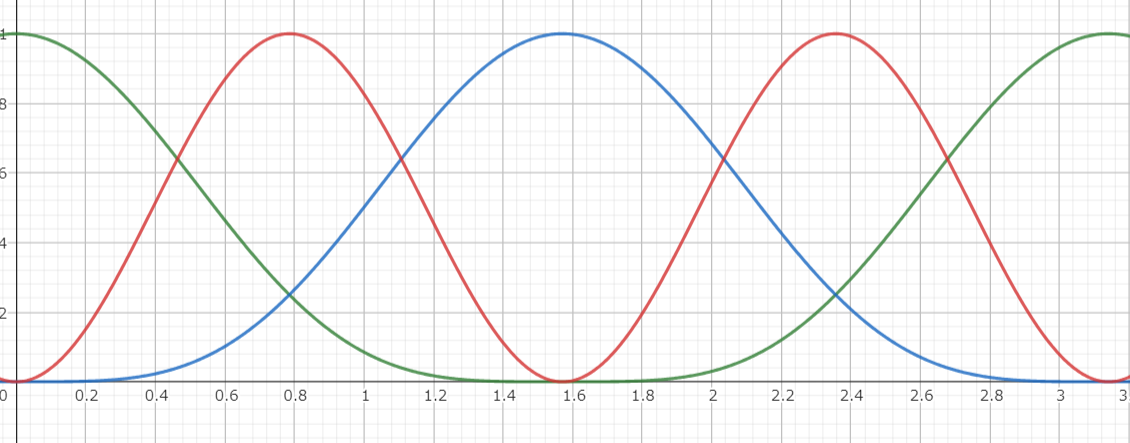
\includegraphics[width=100mm]{image.png}
  \caption{それぞれの様子.緑が$P_0(t)$,青が$P_2(t)$,緑が$P_1(t)$}
  \end{center}
\end{figure}
  

\end{document}